\documentclass[10pt]{article}

\usepackage[letterpaper,hmargin=1.25in,vmargin=1in]{geometry}
\usepackage[T1]{fontenc}
\usepackage{amsmath,amsthm}
\usepackage{newtxtext,newtxmath}
\usepackage{microtype}
\usepackage{xcolor}
\usepackage{graphicx}
\usepackage{booktabs}
\usepackage{mathtools}
\usepackage{fontawesome5}
\usepackage[hidelinks]{hyperref}
\usepackage{enumitem}
\usepackage{titlesec}
\usepackage[font=small,labelfont={bf,color=DeepBlue}]{caption}

\definecolor{DeepBlue}{HTML}{093C4C}
\definecolor{Cyan}{HTML}{087F9A}
\definecolor{Orange}{HTML}{B96722}
\definecolor{SoftBlue}{HTML}{EAF5F7}
\definecolor{SoftRule}{HTML}{9CC8D3}
\definecolor{Body}{HTML}{1D3037}

\hypersetup{colorlinks=true,linkcolor=DeepBlue,citecolor=DeepBlue,urlcolor=Cyan}
\color{Body}
\setlength{\parindent}{0pt}
\setlength{\parskip}{3.2pt}
\setlist{nosep,leftmargin=1.25em}
\titleformat{\section}{\large\bfseries\color{DeepBlue}}{}{0pt}{}[\vspace{-2pt}\color{Cyan}\titlerule]
\titleformat{\subsection}{\normalsize\bfseries\color{DeepBlue}}{}{0pt}{}
\titlespacing*{\section}{0pt}{8pt}{4pt}
\titlespacing*{\subsection}{0pt}{6pt}{2pt}
\newtheoremstyle{aerostat}{4pt}{4pt}{\itshape}{}% space, body
  {\bfseries\color{DeepBlue}}{.}{0.45em}{}
\theoremstyle{aerostat}
\newtheorem{theorem}{Theorem}
\newtheorem{proposition}{Proposition}
\newtheorem{corollary}{Corollary}
\newcommand{\E}{\mathbb E}
\newcommand{\Var}{\operatorname{Var}}
\newcommand{\Skew}{\operatorname{Skew}}
\newcommand{\ExKurt}{\operatorname{ExKurt}}
\newcommand{\RMS}{\operatorname{RMS}}

\begin{document}

\begin{center}
  {\small\href{https://github.com/jonland82/aerostat}{\faGithub\enspace\textbf{Project Repository}}}\par
  \vspace{7pt}
  {\LARGE\bfseries\color{DeepBlue}When Does a Random-Scale Flight Path\par Look Lognormal?}\par
  \vspace{4pt}
  {\large A spherical bridge note from OpenSky trajectories}\par
  \vspace{7pt}
  {\normalsize\textbf{Jonathan R. Landers}}\par
  {\small June 2026}
\end{center}
\vspace{-4pt}

\begin{abstract}
An hour of globally sampled aircraft positions produces a tempting picture: RMS departures from endpoint great-circle arcs are positive, strongly right-skewed, and superficially lognormal. We turn that visual hypothesis into a geometric model. Each deviation is factored as $D=AQ$, where $A$ sets route scale and $Q$ is the RMS shape of an endpoint-pinned bridge. We prove that an independent lognormal scale suppresses the non-Gaussian cumulants of $\log Q$ at explicit rates and give a Wasserstein convergence criterion. For a Brownian bridge, the criterion yields a concrete threshold. Yet the observed log-skewness and kurtosis sharply contradict the resulting single-population prediction. The same theorem that explains a lognormal-looking center therefore diagnoses a distinct near-geodesic boundary population, and a sequential small-ball test estimates when that assignment becomes visible in time. The result is not a universal lognormal law, but a route from visual regularity to a falsifiable mixture model and a time-to-diagnosis statistic.
\end{abstract}

\section{A visual regularity with a geometric question}

The OpenSky Network makes large-scale ADS-B trajectory research possible \cite{schaefer2014}. We sampled 60 one-minute global state snapshots, retained aircraft with all 60 positions, required at least 25 km between endpoints, and removed any track with a one-minute jump above 30 km. The final cohort contains 1,780 tracks. These positions are receiver-dependent observations, not a complete census of global aviation.

For aircraft $i$, write $x_i(t)\in S_R^2$ for its position on the spherical Earth at normalized time $t\in[0,1]$. The direct reference is the minor endpoint geodesic, a standard spherical construction in directional statistics \cite{mardiajupp2000},
\begin{equation}
g_i(s)=\operatorname{Exp}_{x_i(0)}\!\left(s\operatorname{Log}_{x_i(0)}x_i(1)\right),
\qquad s\in[0,1].
\end{equation}
Here $s$ is dimensionless progress, and $g_i(s)$ is a position rather than a distance. If $d_{S_R^2}$ is spherical distance in kilometres, define cross-track displacement and its sampled RMS by
\begin{equation}
\eta_i(t)=d_{S_R^2}\!\left(x_i(t),g_i([0,1])\right),
\qquad
D_i=\left[\frac1{60}\sum_{j=1}^{60}\eta_i(t_j)^2\right]^{1/2}.
\end{equation}
The median $D_i$ is 16.7 km and the mean is 22.7 km. Figure~\ref{fig:deviation} shows why a lognormal model is initially plausible and why that impression is incomplete.

\begin{figure}[ht]
  \centering
  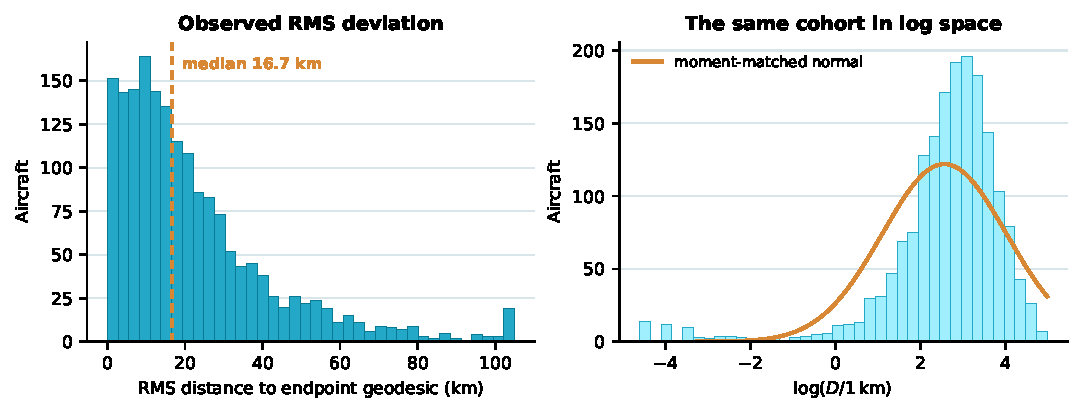
\includegraphics[width=\textwidth]{rms-deviation-distribution.pdf}
  \caption{RMS spherical deviation for the quality-filtered cohort. Left: the application histogram, truncated visually at the 99th percentile while retaining tail observations in the end bin. Right: the 1,776 positive values in log space with a moment-matched Gaussian. The broad center looks compatible with lognormality, but the long lower tail does not.}
  \label{fig:deviation}
\end{figure}

Classical lognormal modeling begins with $\log(D/d_0)\sim N(\mu,\sigma^2)$ for reference distance $d_0=1$ km \cite{aitchison1957}. That describes a shape but supplies no route geometry. We instead ask: \emph{what mechanism makes a spherical path statistic look lognormal, what would falsify it, and how long must one watch before the falsifying boundary component is recognizable?}

\begingroup
\setlength{\fboxsep}{7pt}
\noindent\fcolorbox{SoftRule}{SoftBlue}{%
\begin{minipage}{0.965\textwidth}
\small\raggedright
\textbf{\color{DeepBlue}Narrative arc.}\par\vspace{3pt}
\begin{itemize}[leftmargin=1.15em,itemsep=0pt,topsep=1pt]
\item \textbf{A direct reference.} Aircraft rarely follow the shortest spherical path between observed endpoints, so the endpoint geodesic is a reference rather than an operational route.
\item \textbf{Scale and shape.} Each RMS deviation is written as $D=AQ$: $A$ sets overall magnitude, while $Q$ captures standardized endpoint-pinned shape.
\item \textbf{The smoothing prediction.} Broad variation in $A$ should suppress the skewness and kurtosis contributed by $Q$, making the Brownian product nearly Gaussian in log space.
\item \textbf{The boundary population.} The observed log-skewness is $-2.40$, with 53 tracks at or below $0.1$ km RMS deviation forming a distinct lower-tail boundary.
\item \textbf{Sequential diagnosis.} After the mixture is forced, prefix residuals and Wasserstein gaps ask how long one must watch before assigning a single aircraft to that boundary component.
\end{itemize}
\par
\end{minipage}}
\endgroup

\section{Scale, shape, and the bridge factor}

Factor the observed departure into a kilometre-valued scale and a dimensionless shape,
\begin{equation}
\eta_i(t)=A_iZ_i(t),\qquad
D_i=A_iQ_i,\qquad
Q_i=\left[\int_0^1 Z_i(t)^2\,dt\right]^{1/2},
\end{equation}
where $Z_i(0)=Z_i(1)=0$. Intuitively, $A_i$ asks \emph{how large} the route departure is, while $Z_i$ asks \emph{what shape} it takes between fixed endpoints. Across a population, independent densities $f_A$ and $f_Q$ induce the product law
\begin{equation}
f_D(d)=\int_0^\infty f_A(d/q)f_Q(q)\,\frac{dq}{q}.
\end{equation}
The Jacobian $1/q$ is the signature of multiplicative rather than additive mixing. A single lognormal is therefore not the starting mechanism; it is a possible approximation to this geometry-driven product.

\section{When the product becomes lognormal}

Set $U_\ell=\log(A_\ell/d_0)$ and $V_\ell=\log Q_\ell$ for a sequence of scale-shape populations. The index $\ell$ labels increasing scale dominance, not time or aircraft.

\begin{theorem}[Lognormal smoothing]
Suppose $U_\ell\sim N(\mu_\ell,\sigma_\ell^2)$ is independent of $V_\ell$, with $m_\ell=\E V_\ell$ and $\tau_\ell^2=\Var(V_\ell)<\infty$. Define
\[
W_\ell=\frac{\log(D_\ell/d_0)-(\mu_\ell+m_\ell)}
{\sqrt{\sigma_\ell^2+\tau_\ell^2}}.
\]
If $\tau_\ell^2/(\sigma_\ell^2+\tau_\ell^2)\to0$, then $W_\ell\Rightarrow N(0,1)$. More precisely, for $G_\ell\sim N(m_\ell,\tau_\ell^2)$,
\[
d_{W_2}\!\left(W_\ell,N(0,1)\right)
\leq
\frac{d_{W_2}(V_\ell,G_\ell)}{\sqrt{\sigma_\ell^2+\tau_\ell^2}},
\]
where $d_{W_2}$ is quadratic Wasserstein distance \cite{villani2009}.
\end{theorem}

\begin{proof}
Replace $V_\ell$ by its Gaussian moment match $G_\ell$. Then $U_\ell+G_\ell$ is exactly Gaussian with the displayed centering and variance. Convolution with the same independent $U_\ell$ contracts $W_2$. Finally, independent coupling gives $d_{W_2}(V_\ell,G_\ell)\leq\sqrt{2}\tau_\ell$, so the stated variance ratio forces convergence.
\end{proof}

The theorem formalizes a simple picture: if fleet-to-fleet variation in route scale is broad enough, it blurs the finer distributional signature of route shape.

\begin{proposition}[Exact cumulant attenuation]
For one fixed population, let $\rho=\tau_Q^2/(\sigma_A^2+\tau_Q^2)$, where $\sigma_A^2=\Var(\log(A/d_0))$ and $\tau_Q^2=\Var(\log Q)$. For every $r\geq3$,
\[
\kappa_r(W)=\frac{\kappa_r(\log Q)}{(\sigma_A^2+\tau_Q^2)^{r/2}}.
\]
Consequently,
\[
\Skew(W)=\Skew(\log Q)\rho^{3/2},
\qquad
\ExKurt(W)=\ExKurt(\log Q)\rho^2.
\]
\end{proposition}

\begin{proof}
Independent cumulants add, and a Gaussian has no cumulants above order two. Standardizing by the total log-variance gives the first identity; writing the third and fourth cumulants in standardized form gives the second line.
\end{proof}

These identities turn ``approximately lognormal'' into a checkable statement: shape-induced skewness decays as $\rho^{3/2}$ and excess kurtosis as $\rho^2$.

\section{The Brownian benchmark and its failure}

A standard Brownian bridge is the simplest endpoint-pinned random shape. Its Karhunen--Lo\`eve expansion and RMS functional are
\begin{equation}
Z(t)=\sum_{k=1}^\infty\frac{\sqrt2\,\xi_k}{\pi k}\sin(\pi kt),
\qquad
Q^2=\int_0^1Z(t)^2dt=\sum_{k=1}^\infty\frac{\xi_k^2}{\pi^2k^2},
\end{equation}
with independent $\xi_k\sim N(0,1)$. This is the classical quadratic Brownian-bridge functional underlying Cram\'er--von Mises theory \cite{anderson1952}; its Laplace transform is
\begin{equation}
\E e^{-\lambda Q^2}
=\left(\frac{\sqrt{2\lambda}}{\sinh\sqrt{2\lambda}}\right)^{1/2},
\qquad \lambda>0.
\end{equation}

A two-million-draw, 500-mode numerical evaluation gives
\[
\operatorname{SD}(\log Q)\approx0.385,\qquad
\Skew(\log Q)\approx0.178,\qquad
\ExKurt(\log Q)\approx-0.348.
\]
Substitution in the proposition yields a concrete conclusion: $\sigma_A\gtrsim0.50$ pushes both surviving standardized cumulants below $0.05$ in magnitude. A moderately broad lognormal scale should therefore make this Brownian product look very nearly lognormal.

The observed cohort supplies a sharp diagnostic. Among the 1,776 positive $D_i$ values,
\[
\operatorname{SD}(\log(D/d_0))=1.465,\qquad
\Skew=-2.40,\qquad
\ExKurt=8.11.
\]
Variance matching under the independent Brownian model implies $\sigma_A\approx1.413$. At that scale spread, the proposition predicts skewness about $0.003$ and excess kurtosis about $-0.002$---essentially Gaussian in log space. The data are nowhere close. The mismatch is driven by a near-geodesic boundary: 53 tracks have recorded RMS deviation at or below $0.1$ km.

\section{From an attractive fit to a useful rejection}

The mathematical arc reverses the usual modeling order. We did not choose a flexible mixture merely because a histogram fit was imperfect. Geometry first proposed $D=AQ$; the smoothing theorem then showed that the Brownian single-regime model should be \emph{more} Gaussian in log space than the data; only then did a mixture become necessary.

A natural next model is the finite mixture form \cite{mclachlan2000}
\begin{equation}
f_D(d)=\pi_0 f_0(d)+\sum_{c=1}^{C}\pi_c f_D(d\mid c),
\qquad \pi_c\geq0,\qquad \sum_{c=0}^{C}\pi_c=1,
\end{equation}
where $f_0$ represents the near-geodesic boundary and the continuous components represent distinct route-shape or flight-phase regimes. The current hour cannot identify all such classes, and endpoint geodesics are geometric counterfactuals rather than operationally feasible routes. Those limitations are substantive. Still, the note establishes a clean diagnostic principle: broad lognormal scaling can hide ordinary bridge-shape nonnormality, so a large residual departure is evidence for heterogeneity, dependence, or a boundary mechanism---not merely a slightly misspecified bridge.

\section{Sequential diagnosis of the boundary population}

Once the boundary component has been detected at the cohort level, the next question is individual and temporal: how long must one watch a trajectory before assigning it to that component? Let $C=0$ denote the near-geodesic boundary population and $C=1$ the ordinary bridge population. For the first $n$ samples define the prefix residual
\begin{equation}
R_n^2=\frac1n\sum_{j=1}^n\eta(t_j)^2,
\qquad
\mathcal F_n=\sigma\{\eta(t_1),\ldots,\eta(t_n)\}.
\end{equation}
For a fixed tolerance $\tau$, persistent small residuals are informative only when they are rare under the ordinary component.

\begin{theorem}[Sequential small-ball diagnosis]
Let $\pi_0=\mathbb P(C=0)$. Suppose that, for some $\tau>0$,
\[
\mathbb P_1(R_n\leq\tau)\leq e^{-nI(\tau)}
\qquad\hbox{and}\qquad
\mathbb P_0(R_n\leq\tau)\geq1-\beta_n .
\]
Then
\[
\mathbb P(C=0\mid R_n\leq\tau)
\geq
\frac{\pi_0(1-\beta_n)}
{\pi_0(1-\beta_n)+(1-\pi_0)e^{-nI(\tau)}}.
\]
In particular, posterior confidence $1-\alpha$ is reached once
\[
n\gtrsim
\frac{
\log((1-\pi_0)/\pi_0)+\log((1-\alpha)/\alpha)}
{I(\tau)}
\]
up to the boundary miss term $\beta_n$.
\end{theorem}

\begin{proof}
Bayes' rule gives
\[
\mathbb P(C=0\mid R_n\leq\tau)
=
\frac{\pi_0\mathbb P_0(R_n\leq\tau)}
{\pi_0\mathbb P_0(R_n\leq\tau)+(1-\pi_0)\mathbb P_1(R_n\leq\tau)}.
\]
The two displayed assumptions give the bound. Solving the same inequality for $n$ gives the stated waiting-time scale.
\end{proof}

This is the time-series version of the mixture conclusion: not every straight-looking prefix is diagnostic, but persistent near-zero residual energy becomes decisive once ordinary bridges have too little small-ball mass left.

\begin{figure}[ht]
  \centering
  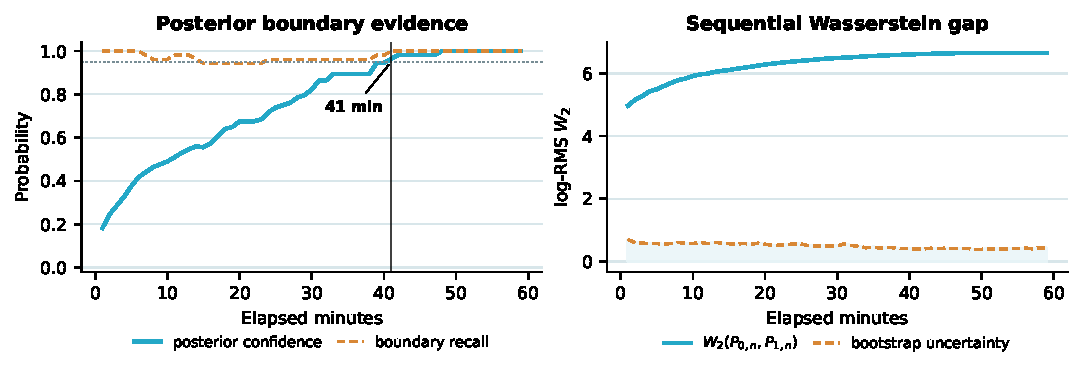
\includegraphics[width=\textwidth]{sequential-boundary-detection.pdf}
  \caption{Sequential boundary diagnostics using the final endpoint geodesic as the reference. Left: empirical posterior confidence and boundary recall for the event $R_n\leq0.1$ km. The prior boundary mass is $53/1780$, so early small residuals are not enough; confidence becomes high only after persistence. Right: the empirical Wasserstein gap between the log-prefix RMS laws of the boundary and ordinary components, plotted against a bootstrap uncertainty floor.}
  \label{fig:sequential}
\end{figure}

The same idea can be expressed in the transport language already used in the smoothing theorem. Let $Y_n=\log(R_n/d_0)$, and let $P_{0,n}$ and $P_{1,n}$ be the laws of $Y_n$ under the boundary and ordinary components. Define
\[
\Delta_n=W_2(P_{0,n},P_{1,n}).
\]
A conservative critical time is
\[
T_W=\inf\{n:\Delta_n>r_{0,n}(\alpha)+r_{1,n}(\alpha)+m\},
\]
where $r_{c,n}(\alpha)$ are sampling radii and $m$ is a chosen margin. For one observed aircraft with value $y_n$, the point-to-law score
\[
S_n(y_n)
=
W_2^2(\delta_{y_n},P_{1,n})
-W_2^2(\delta_{y_n},P_{0,n})
\]
is positive when the observation is closer to the boundary law than to the ordinary law. Thus the practical stopping rule combines individual posterior evidence with population separation:
\[
T_*=\max\{T_{\rm post},T_W\},
\qquad
T_{\rm post}=\inf\{n:\mathbb P(C=0\mid\mathcal F_n)\geq1-\alpha\}.
\]
In the present hour, with $\tau=0.1$ km and $\pi_0=53/1780$, the final-endpoint diagnostic crosses high posterior confidence after roughly forty-one elapsed minutes. The online problem without the final endpoint is harder, because many ordinary trajectories are locally straight; that distinction is exactly what the waiting-time theorem is meant to expose.

\vspace{-3pt}
\begin{thebibliography}{9}\small
\setlength{\itemsep}{0pt}
\setlength{\parskip}{0pt}
\bibitem{schaefer2014}
M. Sch\"afer, M. Strohmeier, V. Lenders, I. Martinovic, and M. Wilhelm,
``Bringing up OpenSky: A large-scale ADS-B sensor network for research,''
\emph{Proc. 13th ACM/IEEE IPSN}, pp. 83--94, 2014.
\href{https://doi.org/10.1109/IPSN.2014.6846743}{doi:10.1109/IPSN.2014.6846743}.

\bibitem{mardiajupp2000}
K. V. Mardia and P. E. Jupp,
\emph{Directional Statistics}.
Wiley, 2000.
\href{https://doi.org/10.1002/9780470316979}{doi:10.1002/9780470316979}.

\bibitem{aitchison1957}
J. Aitchison and J. A. C. Brown,
\emph{The Lognormal Distribution}.
Cambridge University Press, 1957.

\bibitem{villani2009}
C. Villani,
\emph{Optimal Transport: Old and New}.
Springer, 2009.
\href{https://doi.org/10.1007/978-3-540-71050-9}{doi:10.1007/978-3-540-71050-9}.

\bibitem{anderson1952}
T. W. Anderson and D. A. Darling,
``Asymptotic theory of certain goodness of fit criteria based on stochastic processes,''
\emph{Ann. Math. Statist.}, vol. 23, no. 2, pp. 193--212, 1952.
\href{https://doi.org/10.1214/aoms/1177729437}{doi:10.1214/aoms/1177729437}.

\bibitem{mclachlan2000}
G. J. McLachlan and D. Peel,
\emph{Finite Mixture Models}.
Wiley, 2000.
\href{https://doi.org/10.1002/0471721182}{doi:10.1002/0471721182}.
\end{thebibliography}

\end{document}
